% !TEX root = ./../../_Thesis.tex

% chapter's came and label
\chapter{Background}
\label{chap:Background}

The study of how optical aberrations affect visual experience requires a more thorough understanding of human perception and the wave properties of light. In this chapter, we establish and review some of the theoretical principles that were used in the experimental studies, data analysis, interpretation of the results.

% Sensation and Perception Section
% !TEX root = ./../../_Thesis.tex

% section's Name and Label
\section{Sensation and Perception}
\label{sec:SensationAndPerception}

Sensation and perception are the processes that put us in contact with stimuli from our world --- objects and events \cite{King2012}. Understanding these processes requires comprehending the physical properties of our perception and the study of the corresponding sensor,
%sense organ, 
for example, light and the eye. \citet{Lemma2005} defines some concepts that are necessary to explain how stimulation (\eg, visual information) becomes meaningful perception: (i) {\it stimulus}: a source of physical energy that produces a response in a sense organ; (ii) {\it response}: any reaction of an organism to or in the presence of a stimulus; (iii) {\it transduction}: sequence of operations by which physical energy is transformed into patterns of neural impulses that give rise to sensory experience; (iv) {\it sensation}: process of receiving stimulus energies from external environment and transforming those energies into neural energy; and (v) {\it perception}: process whereby the brain interprets sensations, taking into account past experiences, the context in which the sensation occurs, and emotions.

The steps related to the perception of a visual information are illustrated in Figure \ref{fig:flow}, where light waves reflected from the butterfly act as stimuli to react with our sensory receptors, which convert the energy into neural signals. After that, neural messages travel to the sensory cortex of the brain and become sensations. Finally, the process of perception interprets these sensations and grant us to recognize a butterfly \cite{Zimbardo2012}.

\begin{figure}[h]
	\centering
	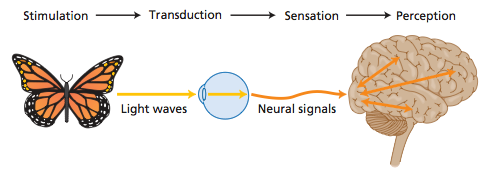
\includegraphics[width=0.73\linewidth]{__Images/02/flow.png}
	\caption[General flow of sensory information]{General flow of sensory information from energy stimulus to sensory receptor cell to sensory neuron to sensation and perception \cite{Zimbardo2012}.}
	\label{fig:flow}
\end{figure}

Light is a form of electromagnetic (EM) radiation which travels through space in waves and can be described in terms of its physical characteristics --- wavelengths and/or amplitude. Color and brightness are the psychological counterparts of light wavelength and intensity that exist only in the brain \cite{King2012}. Humans are capable of detecting only a tiny segment of the EM spectrum, called visible light (Figure \ref{fig:spectrum}), which ranges in wavelength from approximately 400 to 700 nm (1nm = 10$^{-9}$m). 
Wavelengths outside this range are not detected by humans because they are not transmitted by the ocular media or cannot be absorbed by our retinal photopigments \citet{Schwartz2010}.
%Schwartz \citet{Schwartz2010} "other wavelengths are not visible, either because the ocular media does not transmit them or because they are not absorbed by the retinal photopigments".

\begin{figure}[h]
	\centering
	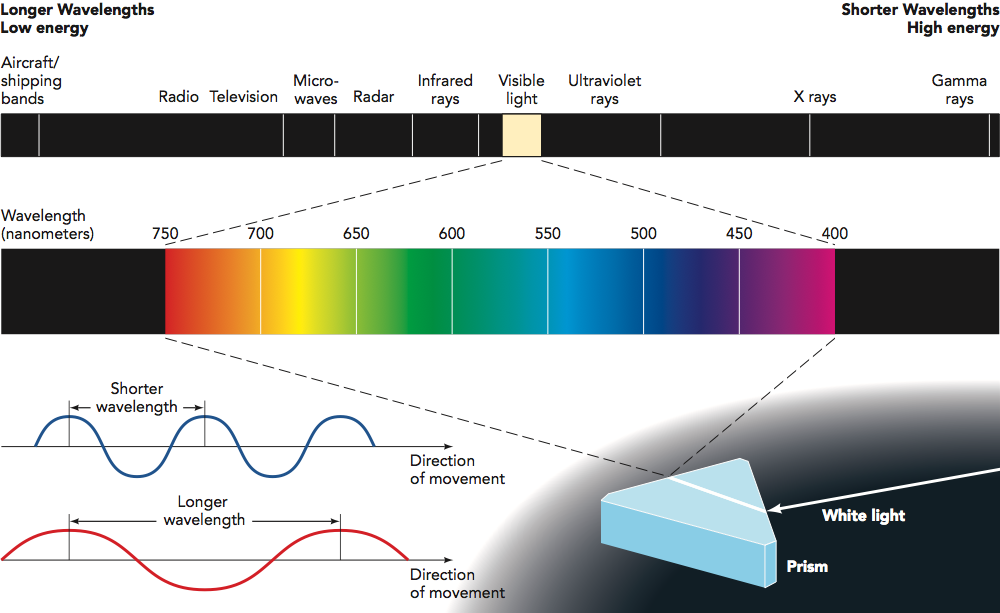
\includegraphics[width=0.95\linewidth]{__Images/02/spectrum.png}
	\caption[The Electromagnetic Spectrum and Visible Light]{The Electromagnetic Spectrum and Visible Light: (Top) Visible light is only a narrow band in the electromagnetic spectrum. Visible light wavelengths range from 400 to 700 nanometers. X rays are much shorter, radio waves much longer. (Bottom) The two graphs show how waves vary in length between successive peaks. Shorter wavelengths are higher in frequency, as reflected in blue colors; longer wavelengths are lower in frequency, as reflected in red colors \cite{King2012}.}
	\label{fig:spectrum}
\end{figure}


%\begin{quote}
%All sensations begins with sensory receptors. Sensory receptors are specialized cells that detect stimulus information and transmit it to sensory nerves and the brain [...] creating local electrical currents. These currents are graded; that means they are sensitive to the intensity of stimulation, such as the difference between a dim and a bright light \cite[p. 80]{King2012}.  
%\end{quote} 
%%\

Distinct neural messages flows into the nervous system as information, and it's type depends on the energy captured by a sensory receptor. Figure \ref{fig:senses} shows the human sensory receptors for vision, hearing, touch, smell, and taste. In order to generate a sensory experience from any receptor, there is a minimal amount of physical energy needed - known as absolute threshold \cite{Zimbardo2012}.

\begin{figure}[h]
	\centering
	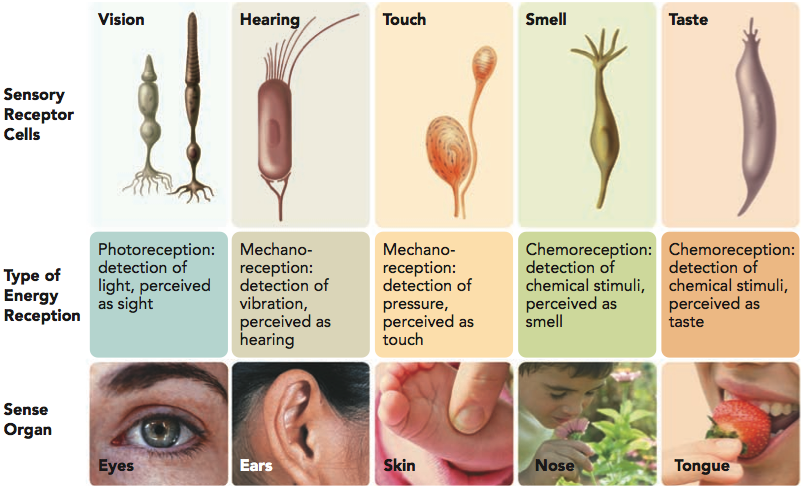
\includegraphics[width=0.95\linewidth]{__Images/02/senses.png}
	\caption[Human Senses: organs, energy stimuli, and sensory receptors]{Human Senses: organs, energy stimuli, and sensory receptors \cite{King2012}.}
	\label{fig:senses}
\end{figure}

Table \ref{table:threshold} shows some typical absolute threshold levels for several familiar stimuli. Experiments designed to determine thresholds, and the study of the relationship between physical nature of stimuli and people's response to them belong to a branch of psychology called {\it psychophysics} \cite{Lemma2005}.

\begin{table}[h]
	\caption[Sensory threshold of five senses]{Sensory threshold of five senses \cite{Zimbardo2012}.}
	\begin{center}
	\begin{tabular}{l l}
	
		\textbf{Sense}	&	\textbf{Detection Threshold} \\
		\hline
		Sight			&	A candle flame at 30 miles on a clear, dark night\\
		Hearing			&	The tick of a watch 20 feet away in a quiet room\\
		Smell			&	One drop of perfume diffused throughout a three-room apartment\\
		Taste			&	One teaspoon of sugar in 2 gallons of water\\
		Touch			&	A bee's wing falling on the cheek from 1 centimeter above\\
	\end{tabular}
	\end{center}
	\label{table:threshold}
\end{table}

%According to \citet{Blake2005}, "understanding perception also makes it possible to design devices to help individuals with impaired sensory function". The following sections focus on aspects of sensation and perception concerning the visual system, and details psychophysical methods for studying perception that could be used to improve individual's visual experience.

% Psychophysics Section
% !TEX root = ./../../_Thesis.tex

% section's Name and Label
\section{Psychophysics}
\label{sec:Psychophysics}


The term \emph{psychophysics} was invented in 1860 by Gustav Theodor Fechner, a German physicist and philosopher, as a mathematical approach to relate mental and physical events on the basis of experimental data \cite{Treutwein1995}. Generally, all sensory systems are able to detect varying degrees of energy, and psychophysical experiments frequently involve the determination of some absolute threshold. This  is a complicated task because humans are not perfect observers. \citet{Lemma2005} emphasizes that the thresholds determined by experiments or clinical procedures may be influenced by several factors, including decision criteria, attention, motivation, and internal neural noise. Further details about Fechner's original methods for determining absolute thresholds and some recent improvements are discussed in \cite{Klein2001, Leek2001, Blake2005}.


% The Human Eye Section
% !TEX root = ./../../_Thesis.tex

% section's Name and Label
\section{The Human Eye}
\label{sec:TheHumanEye}

The eye is a sophisticated imaging system capable of dynamically adjusting its refractive power to focus at a wide range of depths. Optical aberrations in this imaging system are the main causes of loss of visual acuity. {\it Visual acuity} (\ie, the eye's ability to see fine details) can be determined with an auxiliary chart, in which the individual must resolve its details (\eg, bars and gaps) to recognize targets, such as Snellen or Sloan letters (Figure \ref{fig:visual_acuity}). The ability to distinguish between two details determines the {\it Minimum Angle of Resolution} (MAR). The standard visual acuity for humans is 1 arc minute (one-sixtieth of one degree) \cite{Schwartz2010}. In ophthalmology, visual acuity is commonly recorded in the form of the {\it Snellen fraction}: $VA = D'/D$, where $D'$ is the standard viewing distance (usually 20 feet) and $D$ is the distance at which each letter in the chart line subtends 5 arc minutes. The larger the $D$ value, the worse the vision. The term 20/20 vision is the standard for emmetropes (\ie, at a 20 feet distance, a person with normal vision should be able to read the small 20/20 line on an eye chart).

\begin{figure}[h]

	\centering
	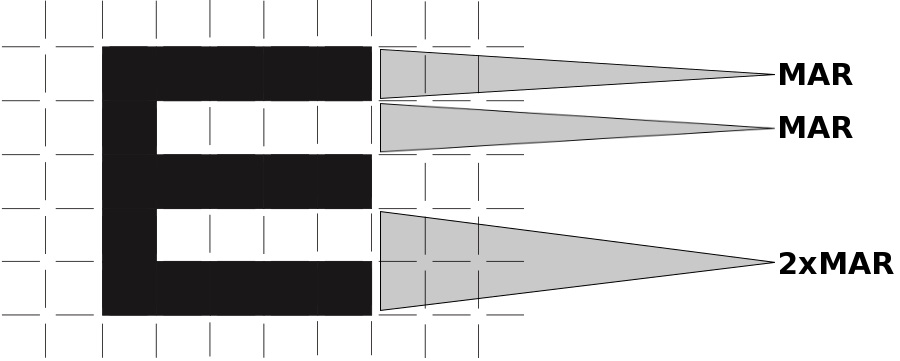
\includegraphics[width=1.0\linewidth]{__Images/02/e_optotype.png}
	\caption[Construction of the optotype E]{Construction of the optotype E. The detail (a bar or a gap) is one-fifth of the overall size of the optotype. MAR stands for Minimum Angle of Resolution, which corresponds to 1 arc minute. Modified from \citet{Schwartz2010}.}
	\label{fig:visual_acuity}
\end{figure}

	% Anatomy Subsection
	% !TEX root = ./../../_Thesis.tex

% subsection's Name and Label
\subsection{Anatomy}
\label{subsec:Anatomy}

The human eye is constituted of several tissues, which contains approximately 126 million receptors cells \cite{King2012}. It can be divided into three concentric layers and two chambers, plus the iris, pupil, and lens. In an adult, it has an average length of 25.4 mm. The outermost layer is the {\it sclera}, the middle layer is the {\it uvea}, and the innermost layer is the {\it retina}. Figure \ref{fig:cross_section} shows a cross section an a human eye and its parts.

\begin{figure}[!t]

	\centering
	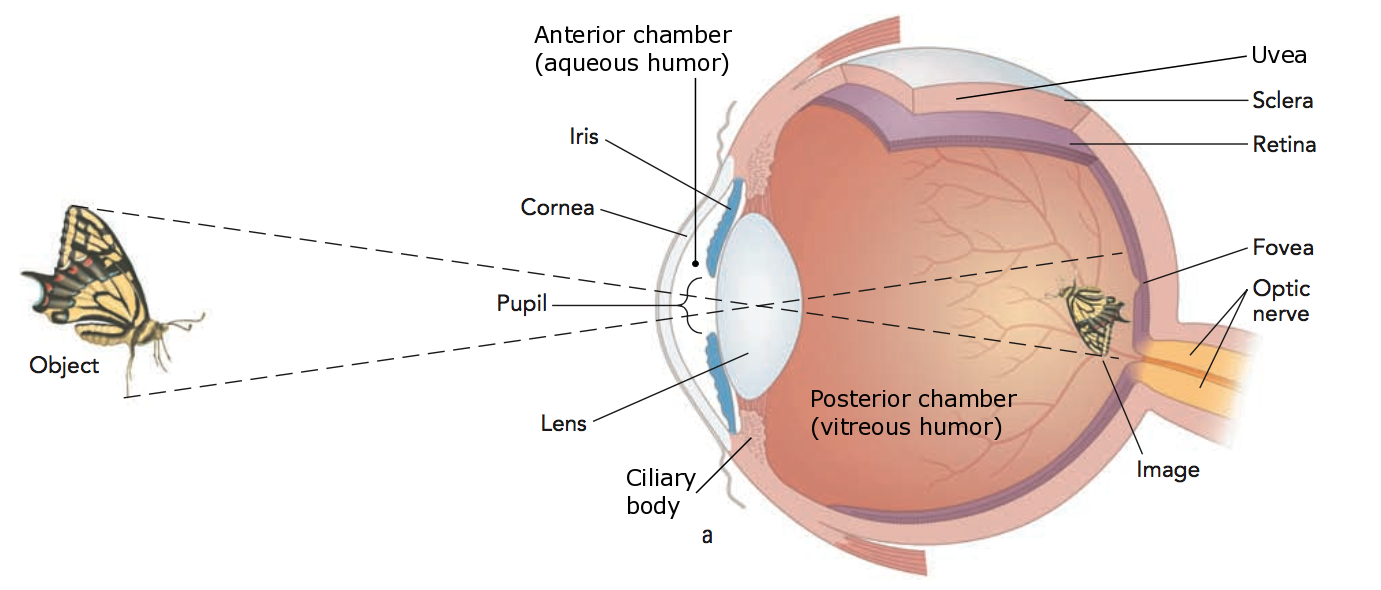
\includegraphics[width=1.00\linewidth]{__Images/02/new-eye.png}
	\caption[Parts of the Eye]{Parts of the Eye. Note that the image of the butterfly on the retina is upside down. The brain allows us to see the image right side up. (modified from \citet{King2012}).}
	\label{fig:cross_section}
\end{figure}

The sclera averages about 1 millimeter in thickness and is made of tightly packed, interwoven fibers that guarantee its toughness. The sclera needs to be tough due to eyeball's pressure, which is the double of the atmospheric pressure \cite{Blake2005}. There is a transparent membrane at the very front of the eye, called {\it cornea}. The cornea is responsible for two-thirds (40 diopters) of the eye's refractive power (total power of 60 diopters) \cite{Tkaczyk2010}. Most part of the uvea layer consists of a heavily pigmented, spongy structure called the {\it choroid}. The choroid averages 0.2 mm thick and contains a network of blood vessels, including capillaries, for blood supply. Its pigmentation reduces light scattering by capturing light that is not captured by the retinal receptor cells. According to \citet{King2012}, the "retina is a light-sensitive surface that records electromagnetic energy and converts it to neural impulses for later processing". It has two kinds of photoreceptors (\ie, light sensitive receptors cells): rods and cones. The retina resembles a very thin, fragile meshwork, which explains its name --- \emph{rete} is Latin for "fisherman's net" \cite{Blake2005}.

Both anterior and posterior chambers contains a specific humor (Figure \ref{fig:cross_section}), which is a transparent liquid continuously produced by the ciliary body. Both aqueous and vitreous humors serve a number of important functions, as maintain the eyeball's shape and nourishment. The iris is the circular section of tissue that gives the eye its characteristic color: brown, blue, green, etc. In the middle of the iris there is 
%a round black region, called pupil. 
the pupil, whose size varies according to the illumination level with the help of two sets of muscles --- the inner and radial \cite{Schwiegerling2004}. Its average diameter varies from 2 millimeters to 8 millimeters, and depends on several factors, such as individual characteristics and luminance level \cite{Yoder2011}.

Right behind the iris, lies an important optical element of the eye, the crystalline lens (see Figure \ref{fig:cross_section}). A gradient-refractive-index lens that contributes approximately one-third (20 diopters) of the dioptric power of the eye, and modifies its shape to focus on near or distant objects \cite{Schwiegerling2004}. This variation, from nearly flat to rounder, causes changes in the final optical power and is called {\it accommodation}. Through accommodation, the lens can correctly focus on the retina the light coming from the scene. For good vision, the crystalline lens must be transparent. %Light must be able to pass through it easily.
Loss of transparency, known as {\it cataracts} leads to a decrease in vision quality
%, called cataracts (\ie, an opacity or reduced transparency of the crystalline lens) 
\cite{Schwartz2010}.

	% Visual Aberrations Section
	% !TEX root = ./../../_Thesis.tex

% section's Name and Label
\subsection{Visual Aberrations}
\label{subsec:VisualAberrations}

Visual aberrations are the main cause of visual impairment. Estimates indicate that there are about 153 million people with visual impairment due to uncorrected refractive errors \cite{Who2007}.
%
\citet{Thibos2002} defined standards for reporting of optical imperfections of eyes. The method of choice for assessing eye aberrations (\ie, describing its wavefront aberration) are the so called {\it Zernike polynomials}. They consist of a series of orthogonal polynomials over the area of a unitary circle (Figure~\ref{fig:unitcircle}) and can be expressed either in Cartesian $(X,Y)$ or polar  $(\theta, \rho)$ coordinate systems. The conversions between the two are given by: 

\begin{equation}
	\label{eq:pol2cart}
	\begin{alignat}{2}
		\rho &= \sqrt{x^2 + y^2}	& \theta &= \tan^{-1}(y/x)  \\
		   x &= \rho*\cos\theta	  &      y &= \rho*\sin\theta
	\end{alignat}
\end{equation}

%\noindent
%where $\rho = r/R$ is the normalized pupil radius.

\begin{figure}[!h]
	\centering
	
\includegraphics[width=0.45\linewidth]{__Images/02/unit_circle.png}
	\caption[The unit circle]{The unit circle.}
	\label{fig:unitcircle}
\end{figure}

There are several different normalization and numbering schemes for representing Zernike polynomials. Here we adopt a double indexing scheme ($Z^{m}_{n}$, where $n$ is the {\it order} and $m$ is the {\it frequency} -- see Figure~\ref{fig:zernike}).
% is useful for unambiguously describing these functions. 
Such a scheme is defined as:

\begin{equation}
	\label{eq:zernikedef}
	\[ Z^m_n(\rho,\theta) = 
		\begin{dcases*} 
			 N^m_n R^{|m|}_n (\rho)\cos m \theta, & for $m$ \geq 0,	\\ 
			-N^m_n R^{|m|}_n (\rho)\sin m \theta, & for $m$ < 0, 
		\end{dcases*} 
	\]
\end{equation}
where $N^m_n$, $R^{|m|}_n$ and the sinusoidal functions stand for the normalization factor, radial component, and azimuthal component, respectively. Such terms are fully described by \citet{Thibos2002}. Some of the {\it Zernike polynomials} (up to the $5^{th}$ order) are listed in Table~\ref{table:Zpoly} and illustrated in Figure~\ref{fig:zernike}. They can be applied directly to wavefront evaluation in the eye's pupil. In ophthalmology, the radial degree $n$ is the basis for classifying aberrations as lower-order ($n\leq2$) and higher-order ($n>2$). However, the vertical and horizontal tilt, as well the zeroth-order piston polynomial, are not considered in measurements of image focus quality \cite{Meister2010}.

%In Figure~\ref{fig:zernike}, it is possible to see some of those polynomials, which can be applied directly to wavefront evaluation in the eye's pupil. In ophthalmology, the radial degree $n$ is the basis for classifying aberrations as lower-order ($n\leq2$) and higher-order ($n>2$). 

\begin{table}[!b]
\centering
\caption{Zernike polynomials up to the fifth order.}
\label{table:Zpoly}
\begin{tabular}{cccll}
\hline
{\bf j} & {\bf n} & {\bf m} & {\bf Zernike Polynomials}	& {\bf Name}	\\ \hline

0	& 0	& 0		& $1$                            					& piston							\\
1	& 1	& -1	& $2\rho \sin\theta $								& vertical tilt						\\
2	& 1	& 1		& $2\rho \cos\theta $								& horizontal tilt					\\
3	& 2	& -2	& $\sqrt{6}\rho^2 \sin\theta$						& oblique astigmatism				\\
4	& 2	& 0		& $\sqrt{3}(2\rho^2-1)$								& defocus							\\
5	& 2	& 2		& $\sqrt{6}\rho^2 \cos\theta $						& vertical astigmatism				\\
6	& 3	& -3	& $\sqrt{8}\rho^3 \sin3\theta$ 						& vertical trefoil					\\
7	& 3	& -1	& $\sqrt{8}(3\rho^3-2\rho)\sin\theta$				& vertical coma						\\
8	& 3	& 1		& $\sqrt{8}(3\rho^3-2\rho)\cos\theta$				& horizontal coma					\\
9	& 3	& 3		& $\sqrt{8}\rho^3 \cos3\theta$						& oblique trefoil					\\
10	& 4	& -4	& $\sqrt{10}\rho^4 \sin4\theta$						& oblique quadrafoil				\\
11	& 4	& -2	& $\sqrt{10}(4\rho^4-3\rho^2)\sin2\theta$			& oblique secondary astigmatism		\\
12	& 4	& 0		& $\sqrt{5}(6\rho^4-6\rho^2+1)$						& primary spherical					\\
13	& 4	& 2		& $\sqrt{10}(4\rho^4-3\rho^2)\cos2\theta$			& vertical secondary astigmatism	\\
14	& 4	& 4		& $\sqrt{10}\rho^4 \cos4\theta$						& vertical quadrafoil				\\
15	& 5	& -5	& $\sqrt{12}\rho^5 \sin5\theta$						& vertical pentafoil				\\
16	& 5	& -3	& $\sqrt{12}(5\rho^5-4\rho^3)\sin3\theta$			& vertical secondary trefoil		\\
17	& 5	& -1	& $\sqrt{12}(10\rho^5-12\rho^3+3\rho)\sin\theta$	& vertical secondary coma			\\
18	& 5	& 1		& $\sqrt{12}(10\rho^5-12\rho^3+3\rho)\cos\theta$	& horizontal secondary coma			\\
19	& 5	& 3		& $\sqrt{12}(5\rho^5-4\rho^3)\cos3\theta$			& oblique secondary trefoil			\\
20	& 5	& 5		& $\sqrt{12}\rho^5 \cos5\theta$						& oblique pentafoil					\\ \hline
\end{tabular}
\end{table}


\begin{figure}[!t]
	\centering
	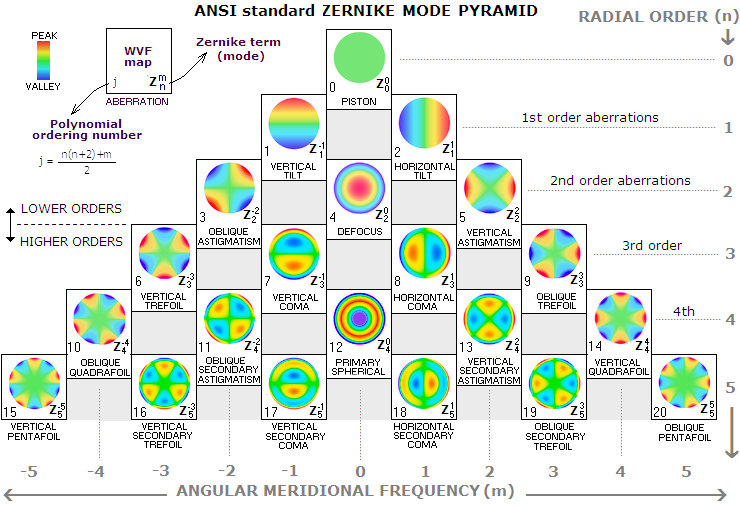
\includegraphics[width=0.98\linewidth]{__Images/02/zernike_pyramide.png}
	\caption[Zernike terms expansion pyramid]{The Zernike expansion pyramid: a function of term's radial degree (or order) $n$ and azimuthal frequency $m$ \cite{Sacek2015}.}
	\label{fig:zernike}
\end{figure}


%When the cornea has an irregularly shape or the eye's axial length is abnormal, light rays bends imperfectly, producing blurry vision. Figure ~\ref{fig:eye_diagram} shows a ray diagram for various eye visual aberrations. Myopic individuals have a natural advantage seeing up close, and objects are formed in front of the retina. Hyperopia causes the exact opposite of myopia and distant objects appear clear and close-up objects appear blurry. Under this condition, the image forms behind the retina. Astigmatism is a low-order aberration caused by a toric curvature in the cornea or crystallin.




% Optics and Wavefront Theory Section
% !TEX root = ./../../_Thesis.tex

% section's Name and Label
\section{Optics and Wavefront Theory}
\label{sec:OpticsAndWavefrontTheory}

The human eye consists of several optical components, notably the cornea, the crystalline lens, the pupil, and the retina. Visual aberrations are the combination of the imperfections/anomalies from the outermost  to the innermost  component. The aim of vision correction is to remove or to minimize the ocular aberrations of the visual system. But to achieve this goal, we first need to understand and analyze how light behaves inside the eye.

%There are two main aspects to how human eye forms images. One is concerned with the physics of image formation and the other with its geometry. We need the former's approach to determine how light waves propagate and behave in the eye, or optical system in general. The geometrical one is a linear interface based on the simplified directional model of light propagation. However, 
According to \citet{Sacek2015} even though \emph{geometrical optics} provides a proper way of determining image location and magnification by tracking paraxial rays, the determination of optical systems' aberrations require more complex calculation considering light waves and its propagation (\ie, \emph{physical optics}).

% O paragrafo e a figura abaixo estão deslocados, sem aparente conexao com o restante do texto
%
%In Figure~\ref{fig:reduced_eyes} it is possible to see two very useful schematic eye models, which allows for a very simple calculation of the refracting power of the entire eye. Both are based in the most influential schematic eye model, constructed by Nobel Laureate Allvar Gullstrand (REF???), and can be used widely used either in geometrical or physical optics.
%
%\begin{figure}[b]
%
	%\centering
	%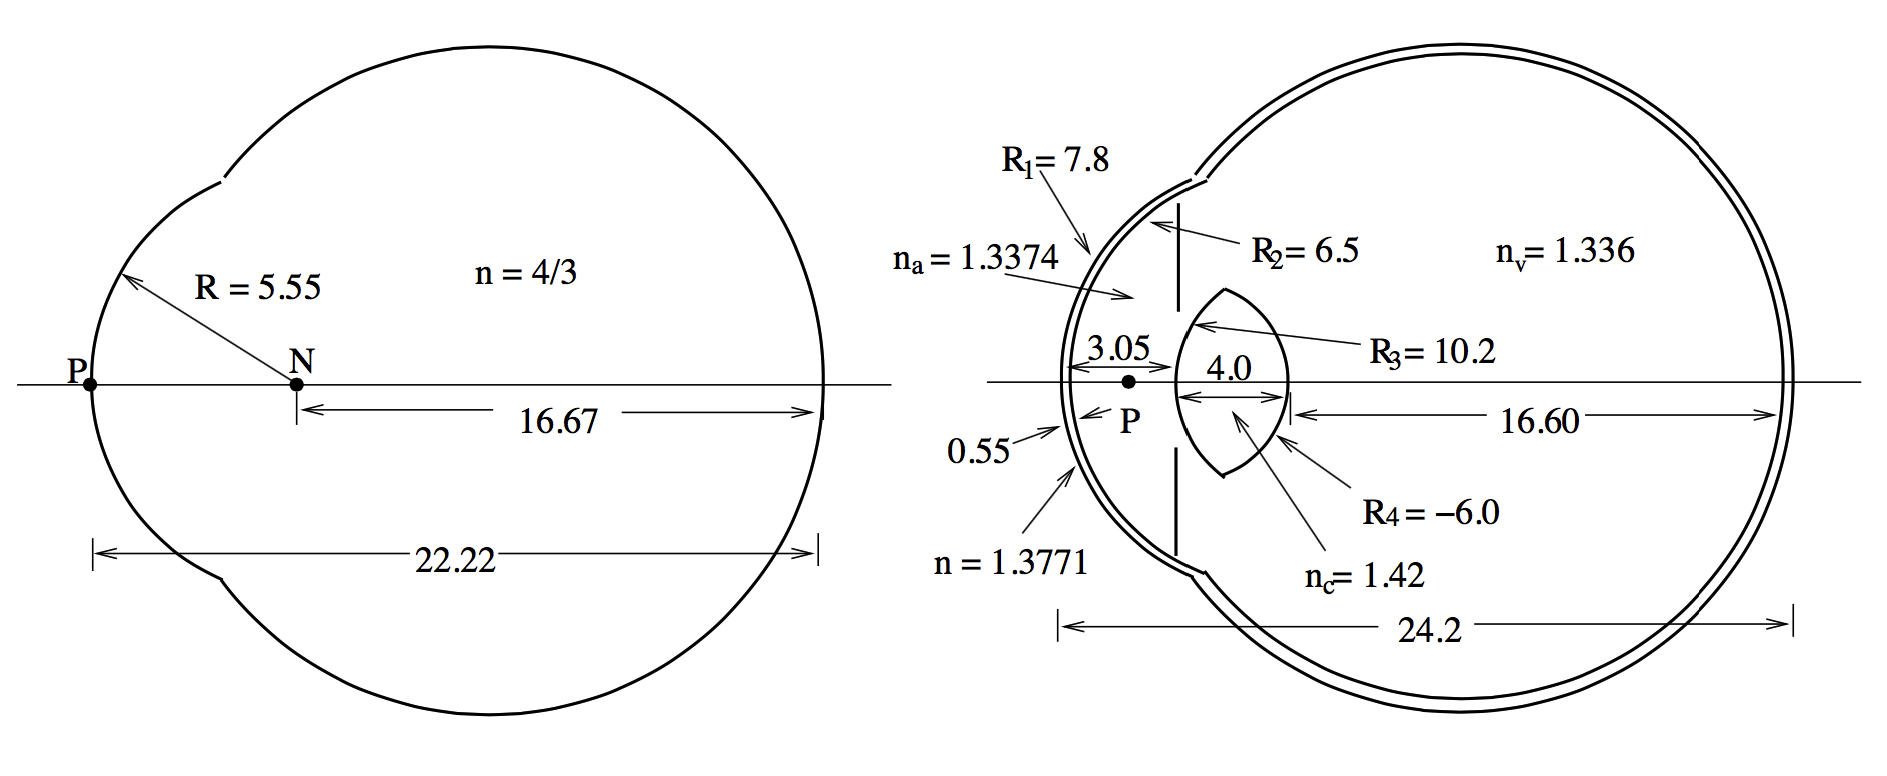
\includegraphics[width=0.95\linewidth]{__Images/02/schematic_eyes.png}
	%\caption[Two very useful schematic eye models]{Two very useful schematic eye models: (right) Emsley reduced schematic eye; (left) Gullstrand-Le Grand theoretical eye. All distance measures are in mm \cite{Dai2008}.}
	%\label{fig:reduced_eyes}
%\end{figure}


\citet{Dai2008} states that "a propagating wavefront can be characterized as many rays propagating in different directions as determined by the local slopes of the wavefront surface". Suppose there is an original wavefront $W(x,y)$, centered at point $O$ and conformed within the aperture $\Sigma$, as shown in Figure~\ref{fig:wavefront_geometry}. When it propagates towards an eye by a distance $d$, it becomes a new wavefront $W'(x',y')$ given as

\begin{equation}
	\centering
	\label{eq:propwave}
	W'(x',y') = W(x,y) + z(x,y;x',y'),
\end{equation}
%	z(x,y;x',y') = \sqrt {d^2+(x-x')^2+(y-y')^2}
\noindent
where $z(x,y;x',y')$ is the distance between points $P(x,y)$ and $P'(x',y')$ (Figure~\ref{fig:wavefront_geometry}), and can be written as:
\begin{equation}
	\centering
	\label{eq:dist}
	z(x,y;x',y') = \sqrt {d^2+(x-x')^2+(y-y')^2}.
\end{equation}

\begin{figure}[!t]

	\centering

	\subfigure[]{
		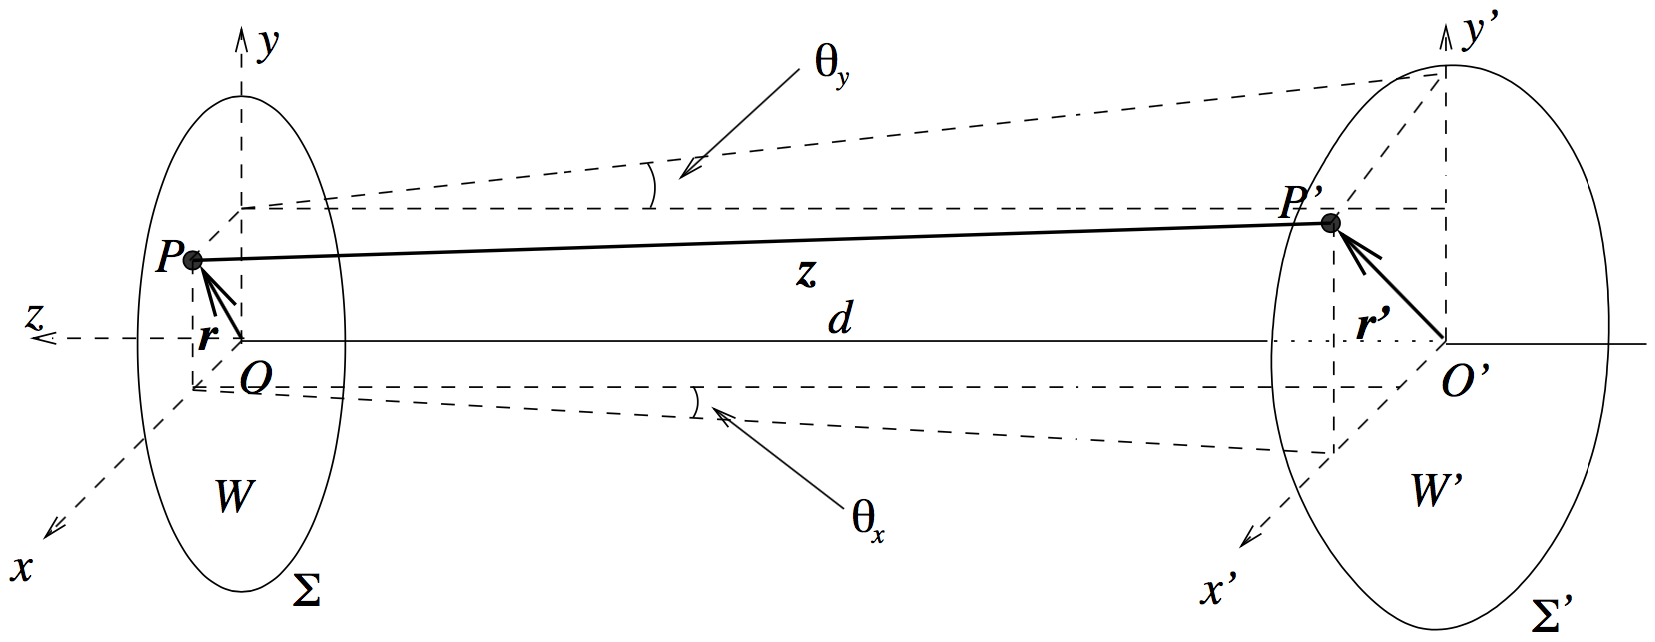
\includegraphics[width=0.7\linewidth]{__Images/02/wavefront_geometry.png}
		\label{fig:wavefront_geometry}
	}
	~
	\subfigure[]{
		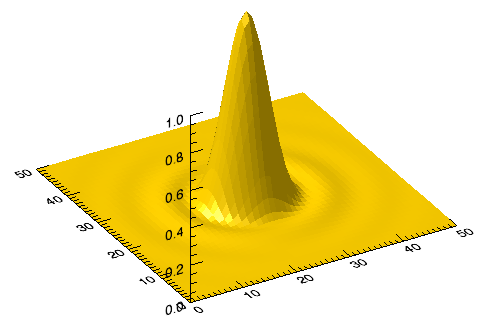
\includegraphics[width=0.25\linewidth, height=10em]{__Images/02/psf_airy3d.png}
		\label{fig:psf_geom}
	}

	\caption[General concepts of wavefront]{General concepts of wavefront: (a) Geometry of the wavefront propagation \cite{Dai2008}; (b) the PSF generated by an aberrated wavefront \cite{Smith2015}.}
	\label{fig:wave_psf}
\end{figure}

The propagation of a wavefront $W(x,y)$ consisting of low-order aberrations only, expressed with Zernike Polynomials, is discussed by \cite{Dai2008}. In addition, the author discusses several optical metrics of ocular wavefronts. A very good predictor for visual performance is the point spread function (PSF), which describes how a ray of light is dispersed in a given space. It is represented by a 2-D array and, as shown in Figure~\ref{fig:psf_geom}, resembles a surface in 3-D. It can be obtained using Fourier Optics \cite{Goodman2005} and the eye's wavefront aberration information. 
% and then used as a 2-D blur filter to be convolved with an image.

\section{Summary}
%
This chapter reviewed the background information about the human eye required for understanding the remaining of this thesis. 

